\section*{Figure Legends}
\label{figures}

\subsubsection*{Figure~\ref{fig:chondrocyte-model}.}
An illustration of the model.


\subsubsection*{Figure~\ref{fig:potassium-currents}.}
Potassium currents which are fit to experimental values (in red) from
\cite{Clarketal2011}. \Ko = 5~mM, \Nao = 140~mM, \Cao = 2~mM, pH = 7.4,
except for $I_{K_{\mathrm{2\; pore}}}$, where \Ko = 145~mM, pH = 8.5.


\subsubsection*{Figure~\ref{fig:other-currents}.}
V-I relations for the other used currents. These are not fit to
experimental data, but used to tune simulation results.

\subsubsection*{Figure~\ref{fig:overall-behaviour}.}
Overall behaviour of the model when voltage is ramped from -130~mV to
+90~mV in 1~s. It validates well with respect to the experimental data.

\subsubsection*{Figure~\ref{fig:concentrations}.}
(Non)Evolution of the concentrations over 1800~s to show that the
initial conditions we have chosen for the model were at steady state.

\subsubsection*{Figure~\ref{fig:varying-Ko}.}
Evolution of membrane potential with varying external potassium
concentration.

\clearpage
\begin{figure}
  \centering
  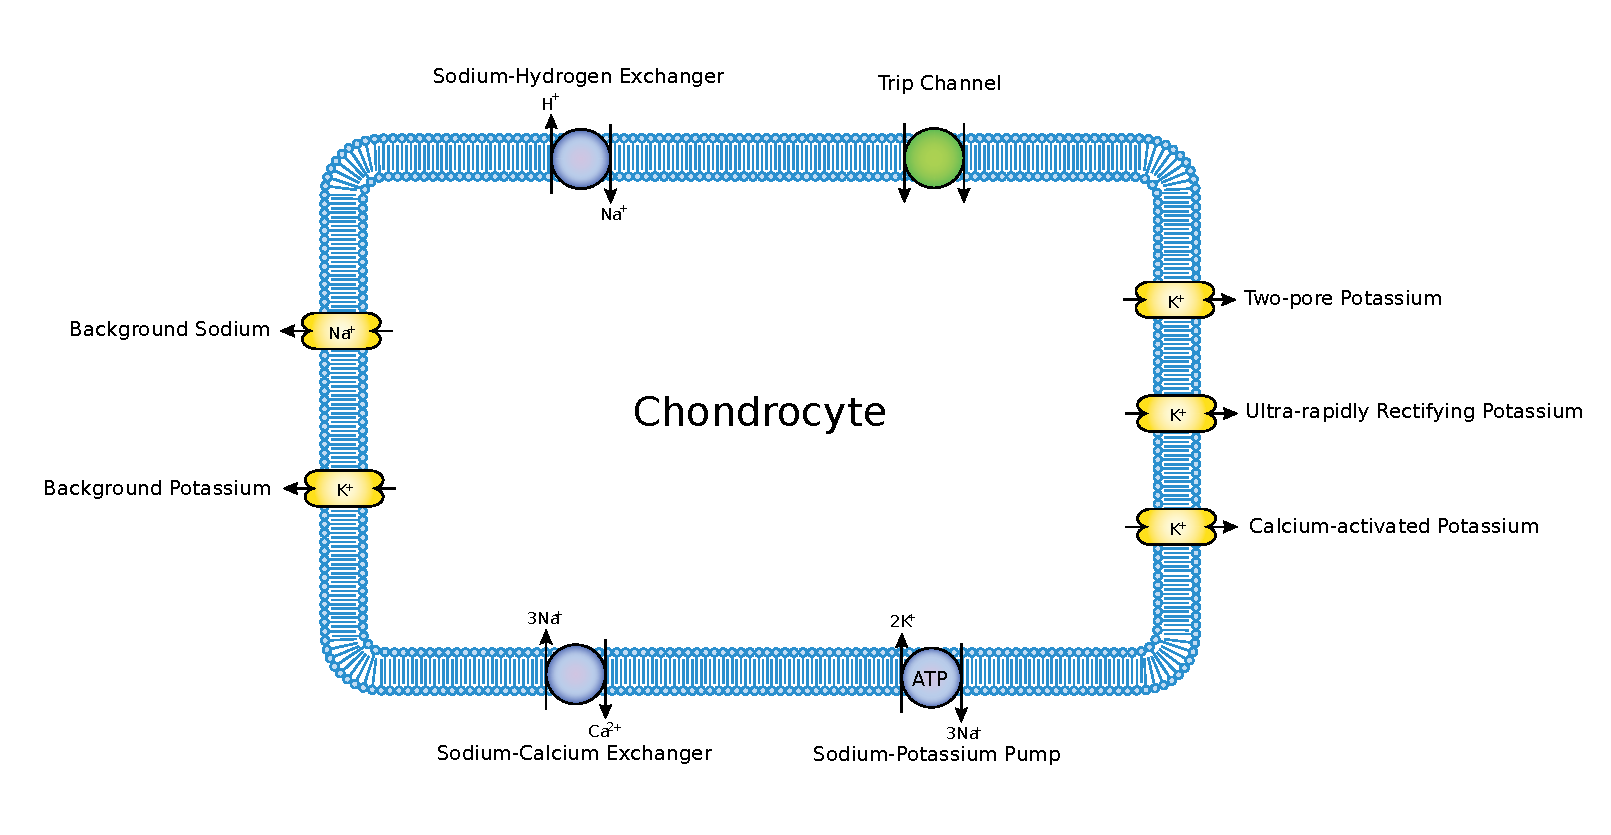
\includegraphics[width=\textwidth]
  {../images/pdf/chondrocyte-model-cellml}
  \caption{}
  \label{fig:chondrocyte-model}
\end{figure}

\clearpage
\begin{figure}
  \centering
  \subfloat{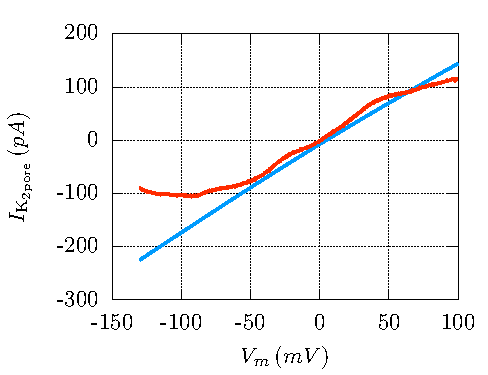
\includegraphics[width=0.5\textwidth]
    {../results/pdf/20120803/V-I_K_2pore}}
  \subfloat{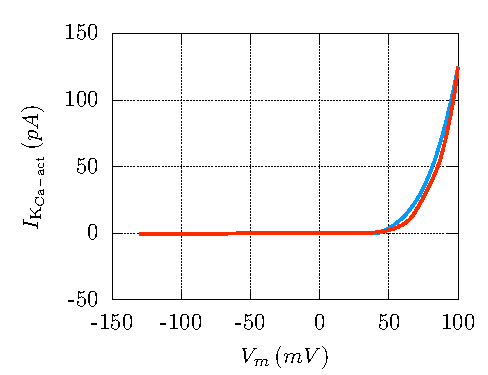
\includegraphics[width=0.5\textwidth]
    {../results/pdf/20120803/V-I_K_Ca_act}}\\
  \subfloat{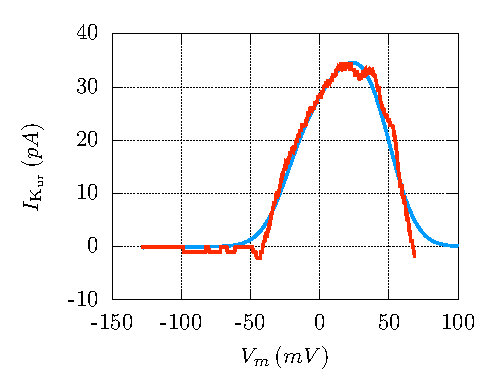
\includegraphics[width=0.5\textwidth]
    {../results/pdf/20120803/V-I_K_ur}}
  \subfloat{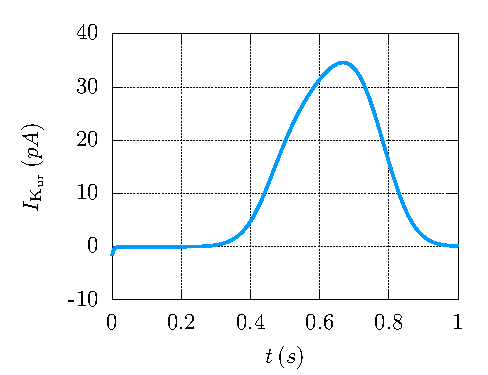
\includegraphics[width=0.5\textwidth]
    {../results/pdf/20120803/t-I_K_ur}}
  \caption{}
  \label{fig:potassium-currents}
\end{figure}

\clearpage
\begin{figure}
  \centering
  \subfloat{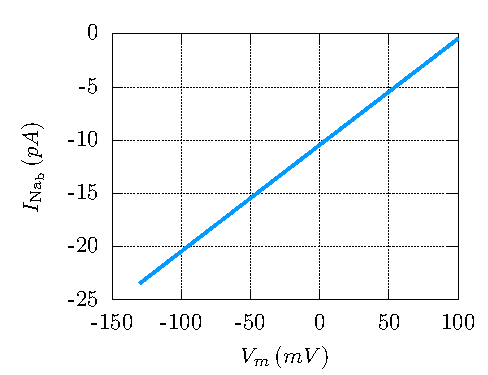
\includegraphics[width=0.5\textwidth]
    {../results/pdf/20120803/V-I_Na_b}}
  \subfloat{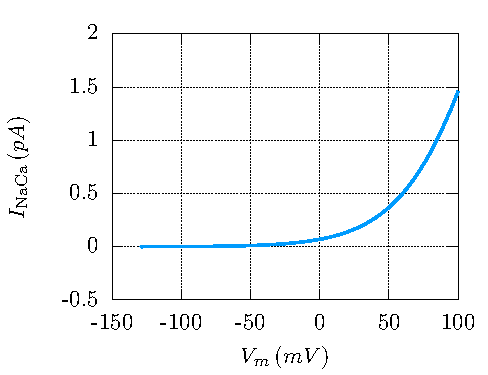
\includegraphics[width=0.5\textwidth]
    {../results/pdf/20120803/V-I_NaCa}}\\
  \subfloat{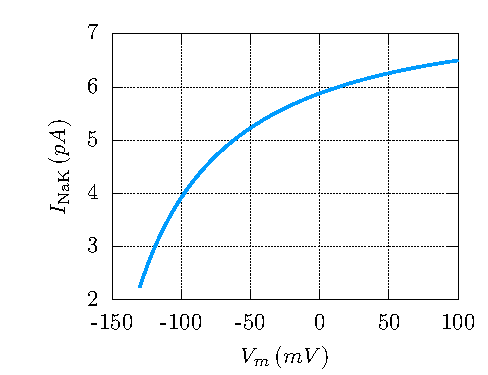
\includegraphics[width=0.5\textwidth]
    {../results/pdf/20120803/V-I_NaK}}
  \subfloat{\hspace{0.5\textwidth}}
  \caption{}
  \label{fig:other-currents}
\end{figure}

\clearpage
\begin{figure}
  \centering
  \subfloat{\includegraphics[width=0.5\textwidth]
    {../results/pdf/20120803/t-v}}
  \subfloat{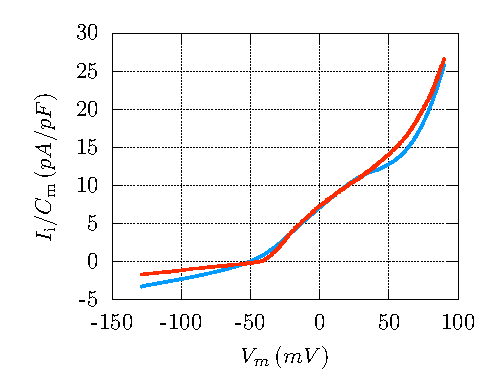
\includegraphics[width=0.5\textwidth]
    {../results/pdf/20120803/V-I_i_by_Cm}}\\
  \subfloat{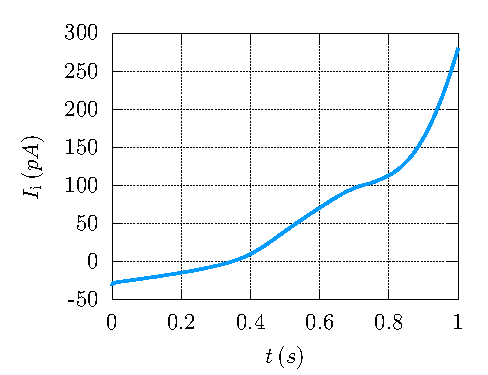
\includegraphics[width=0.5\textwidth]
    {../results/pdf/20120803/t-I_i}}
  \subfloat{\hspace{0.5\textwidth}}
  \caption{}
  \label{fig:overall-behaviour}
\end{figure}

\clearpage
\begin{figure}
  \centering
  \subfloat{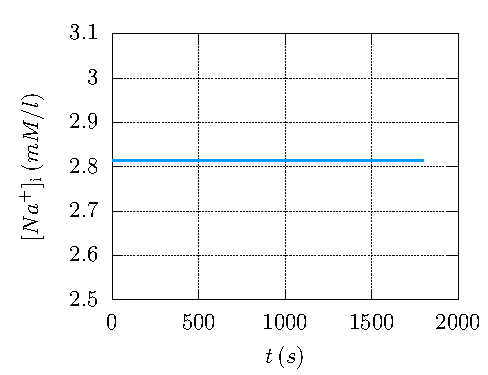
\includegraphics[width=0.50\textwidth]
    {../results/pdf/20120803/t-Na_i}}
  \subfloat{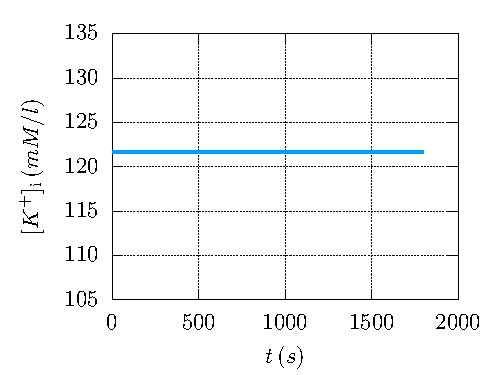
\includegraphics[width=0.50\textwidth]
    {../results/pdf/20120803/t-K_i}}\\
  \subfloat{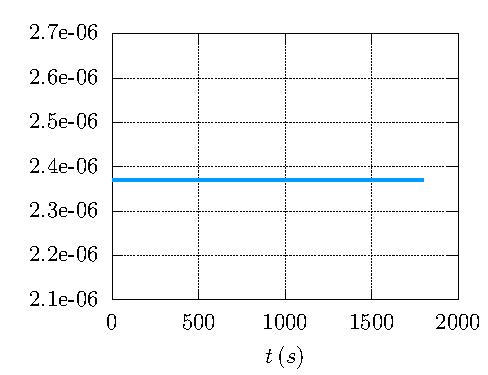
\includegraphics[width=0.50\textwidth]
    {../results/pdf/20120803/t-Ca_i}}
  \subfloat{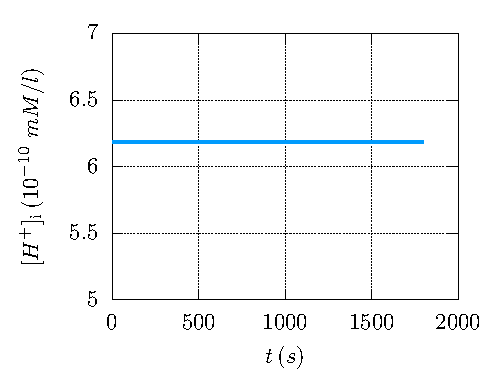
\includegraphics[width=0.50\textwidth]
    {../results/pdf/20120803/t-H_i}}\\
\subfloat{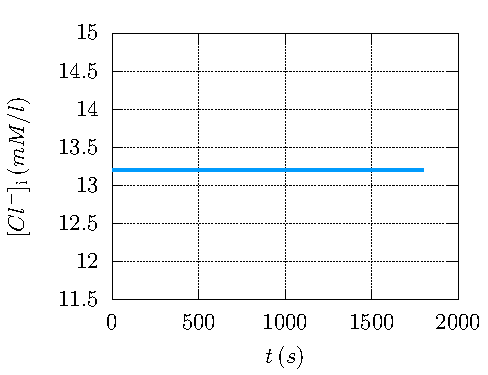
\includegraphics[width=0.50\textwidth]
  {../results/pdf/20120803/t-Cl_i}}
  \subfloat{\hspace{0.50\textwidth}}\\
  \caption{}
  \label{fig:concentrations}
\end{figure}

\clearpage
\begin{figure}
  \centering
  \subfloat[Without BUP]{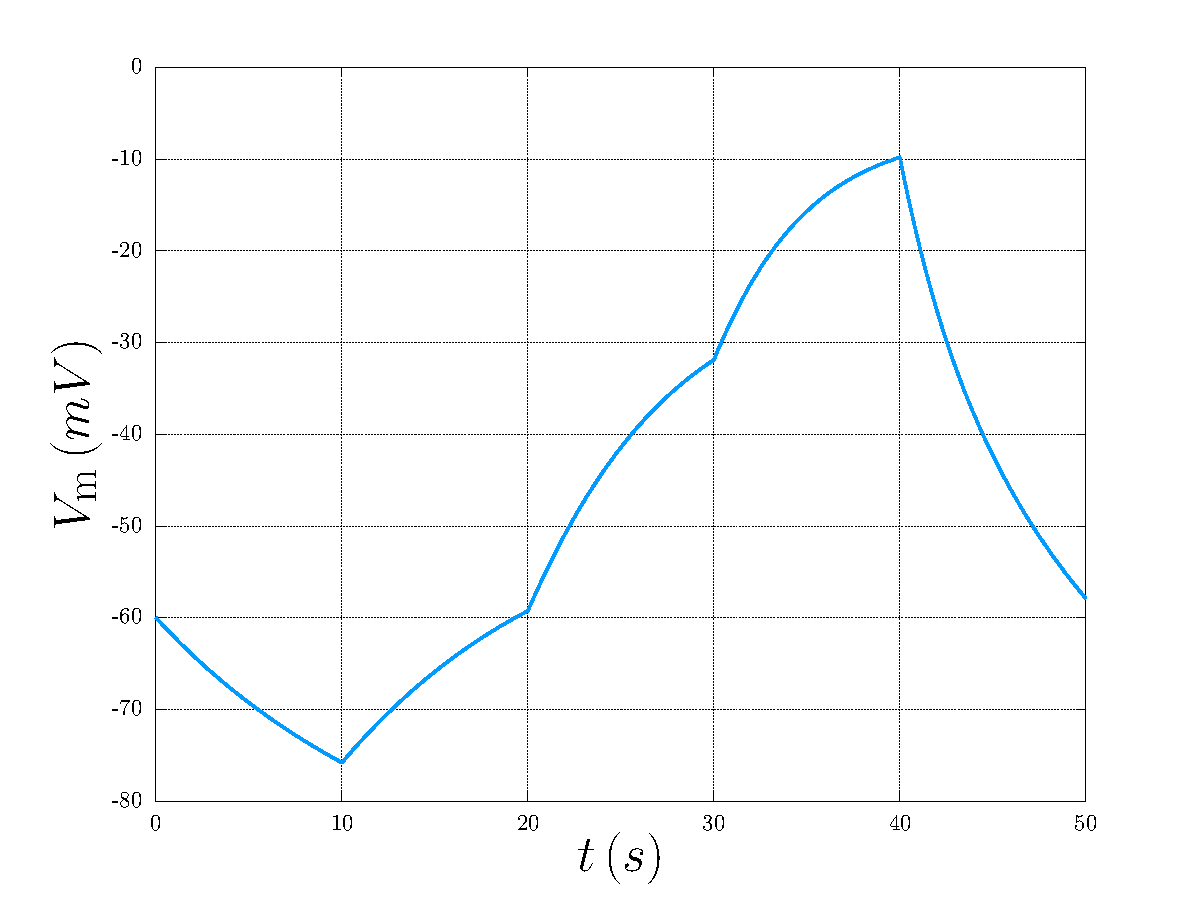
\includegraphics[width=0.5\textwidth]
    {../results/pdf/20110902/t-V-withoutBUP}}
  \subfloat[With BUP]{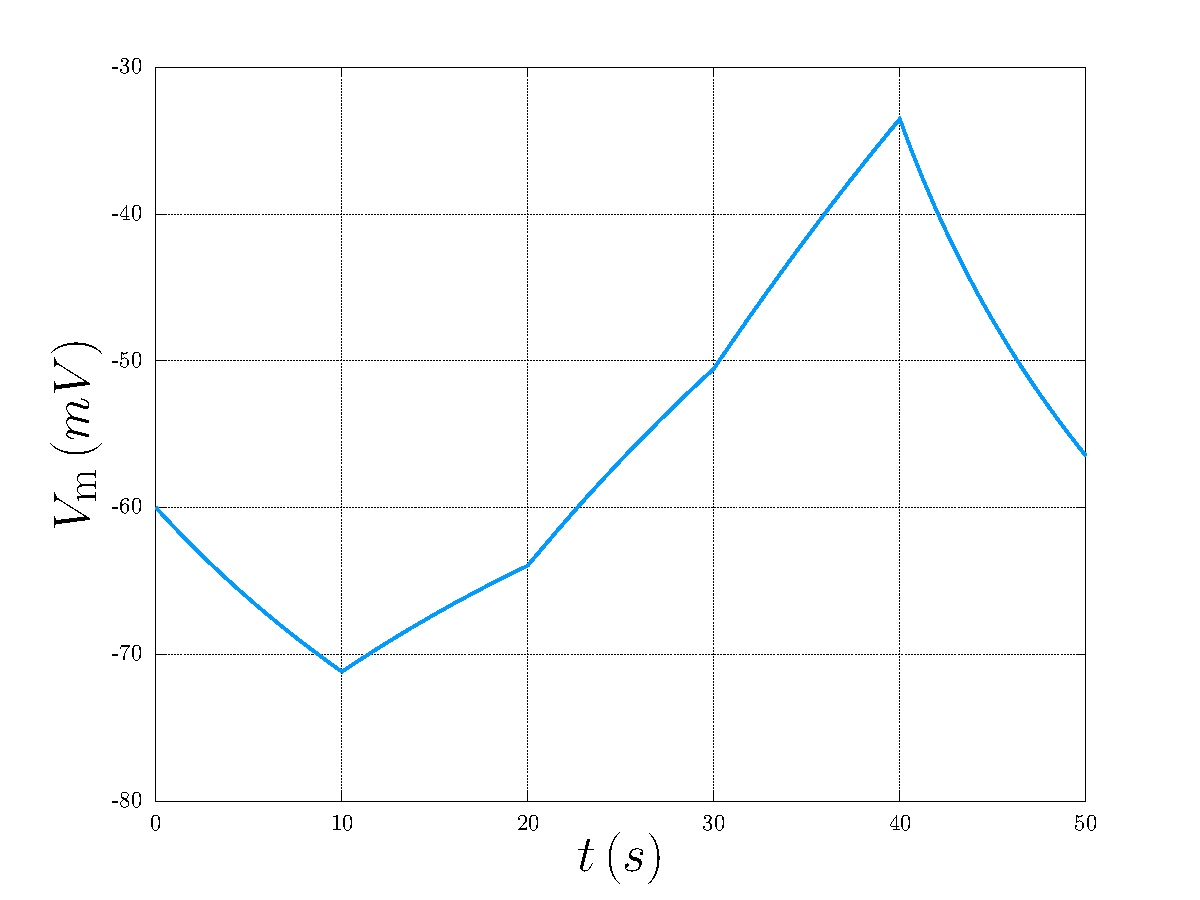
\includegraphics[width=0.5\textwidth]
    {../results/pdf/20110902/t-V-withBUP}}\\
  \subfloat{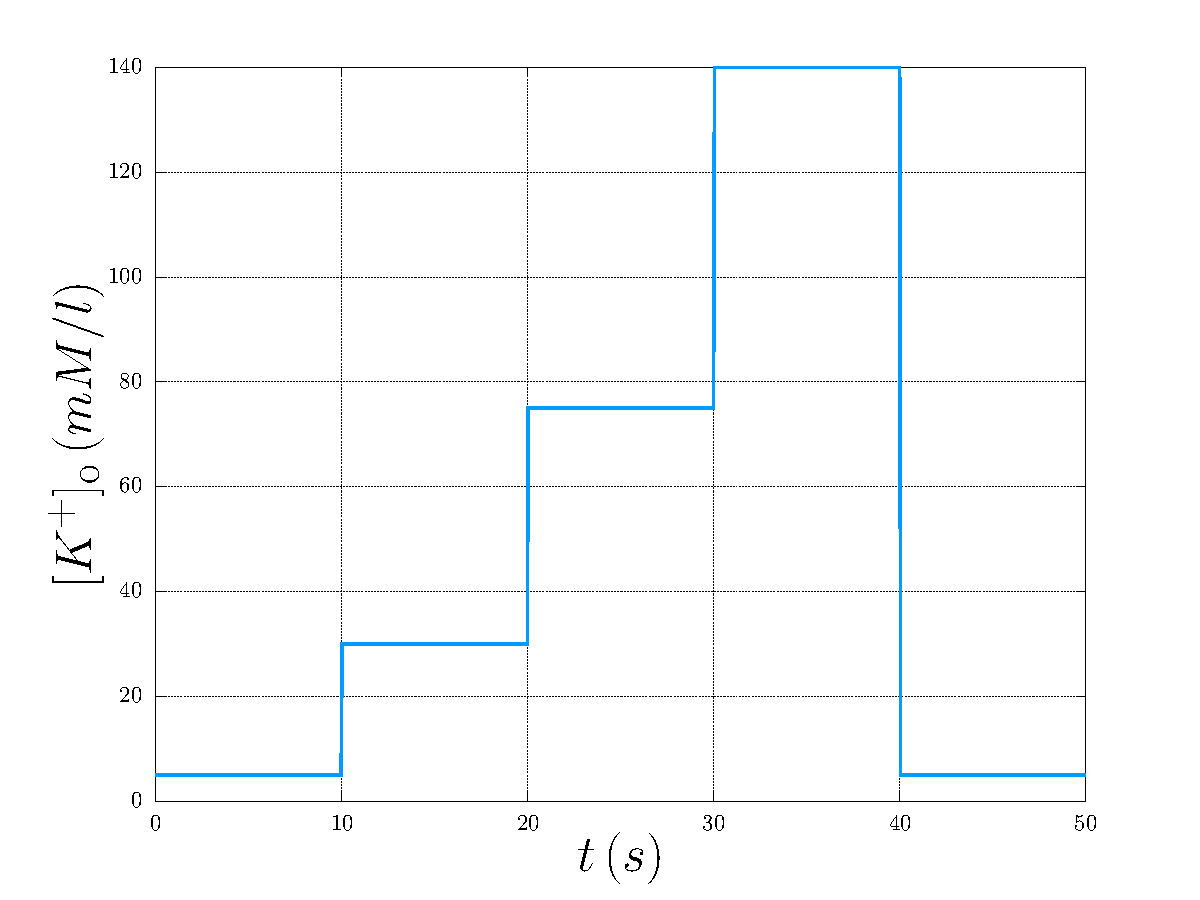
\includegraphics[width=0.5\textwidth]
    {../results/pdf/20110902/t-K_o}}
  \subfloat{\hspace{0.5\textwidth}}
  \caption{}
  \label{fig:varying-Ko}
\end{figure}

% Local Variables:
% TeX-master: "chondrocyte-model"
% mode: latex
% mode: flyspell
% End:
